\begin{figure}
\begin{minipage}[c]{0.95\linewidth}
\begin{minipage}[c]{0.49\textwidth}
  \centering
  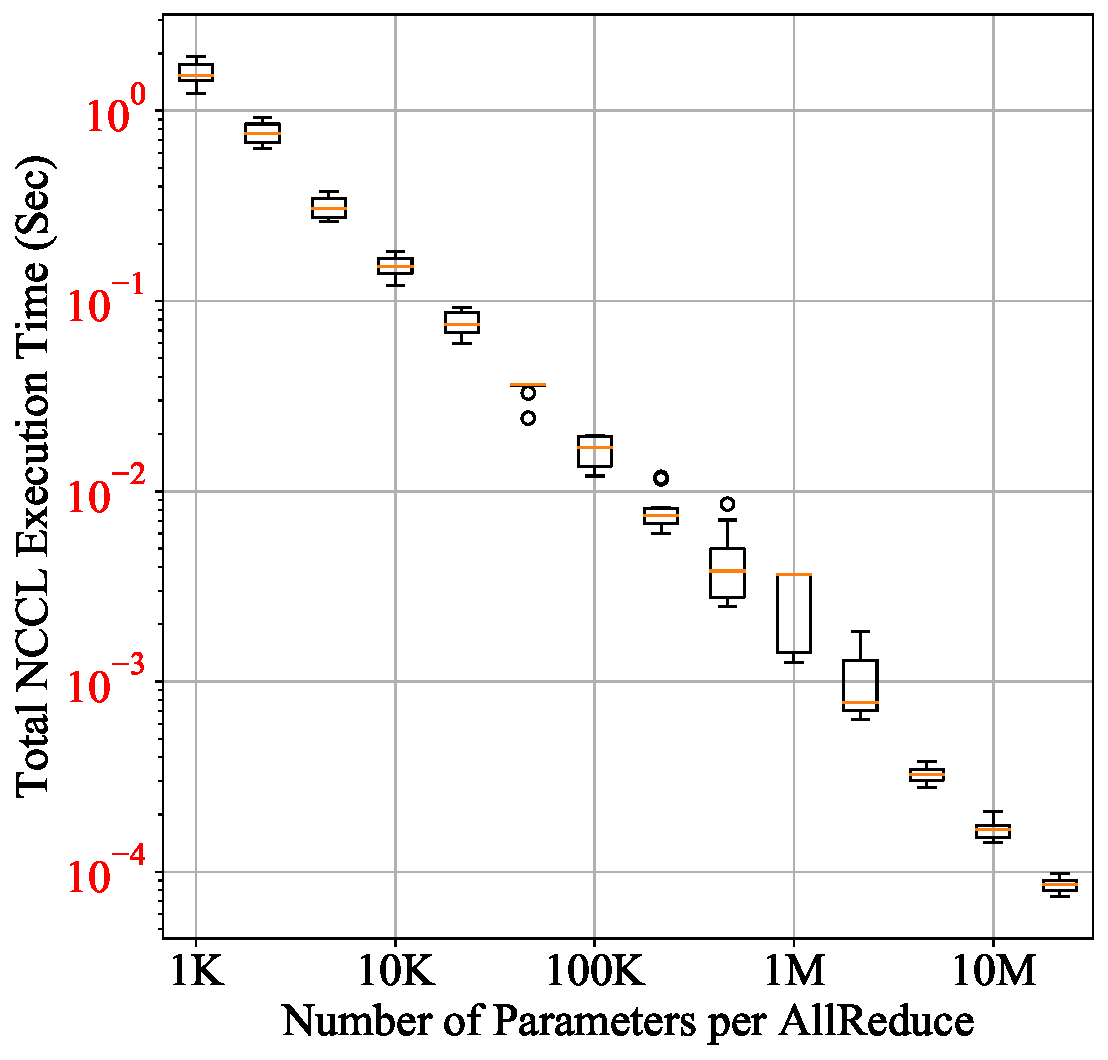
\includegraphics[width=\linewidth]{image/allreduce_nccl.pdf}
  (a) NCCL
\end{minipage}
\begin{minipage}[c]{0.49\textwidth}
  \centering
  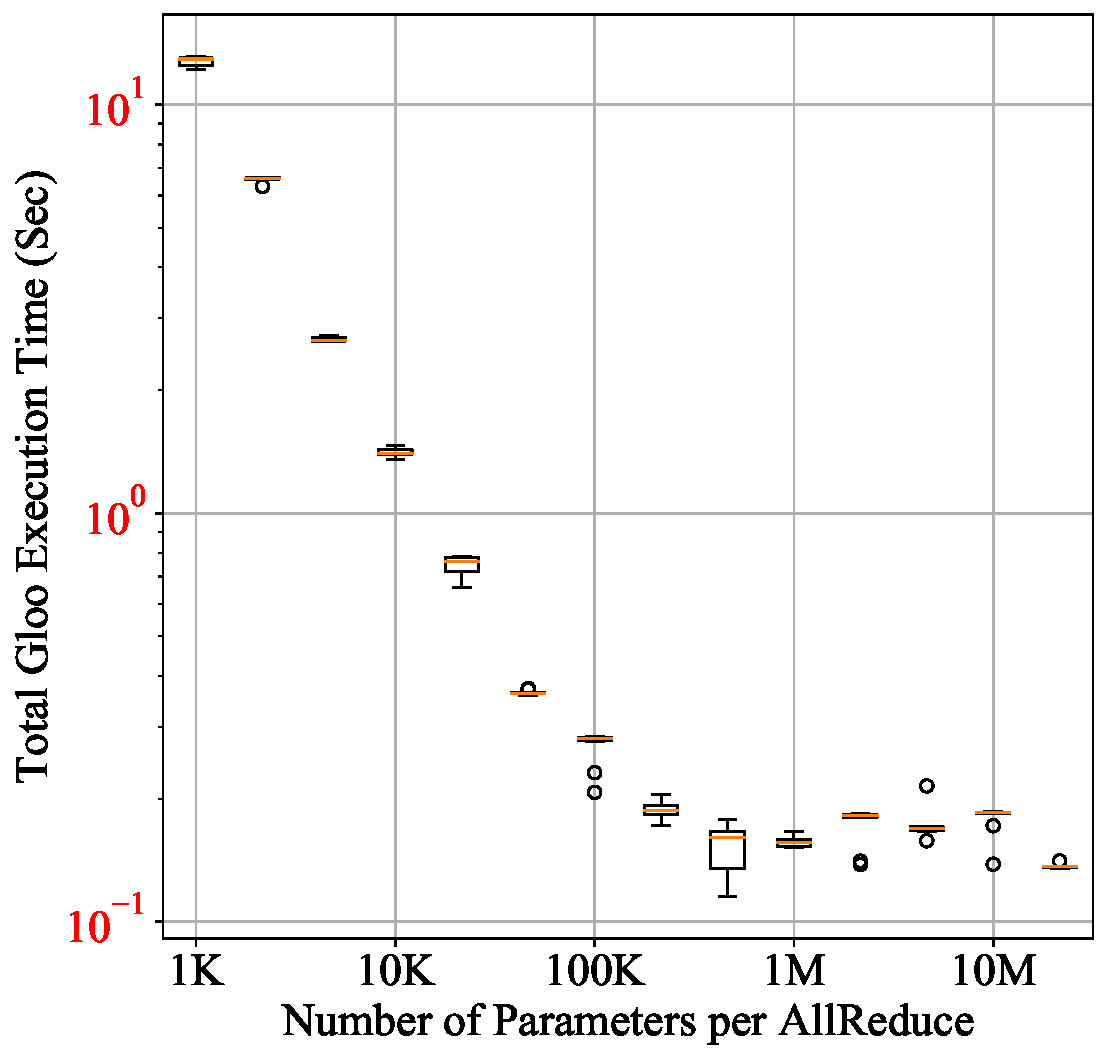
\includegraphics[width=\linewidth]{image/allreduce_gloo.pdf}
  (b) GLOO
\end{minipage}
\end{minipage}
\begin{minipage}[c]{0.95\linewidth}
\begin{minipage}[c]{0.49\textwidth}
  \centering
  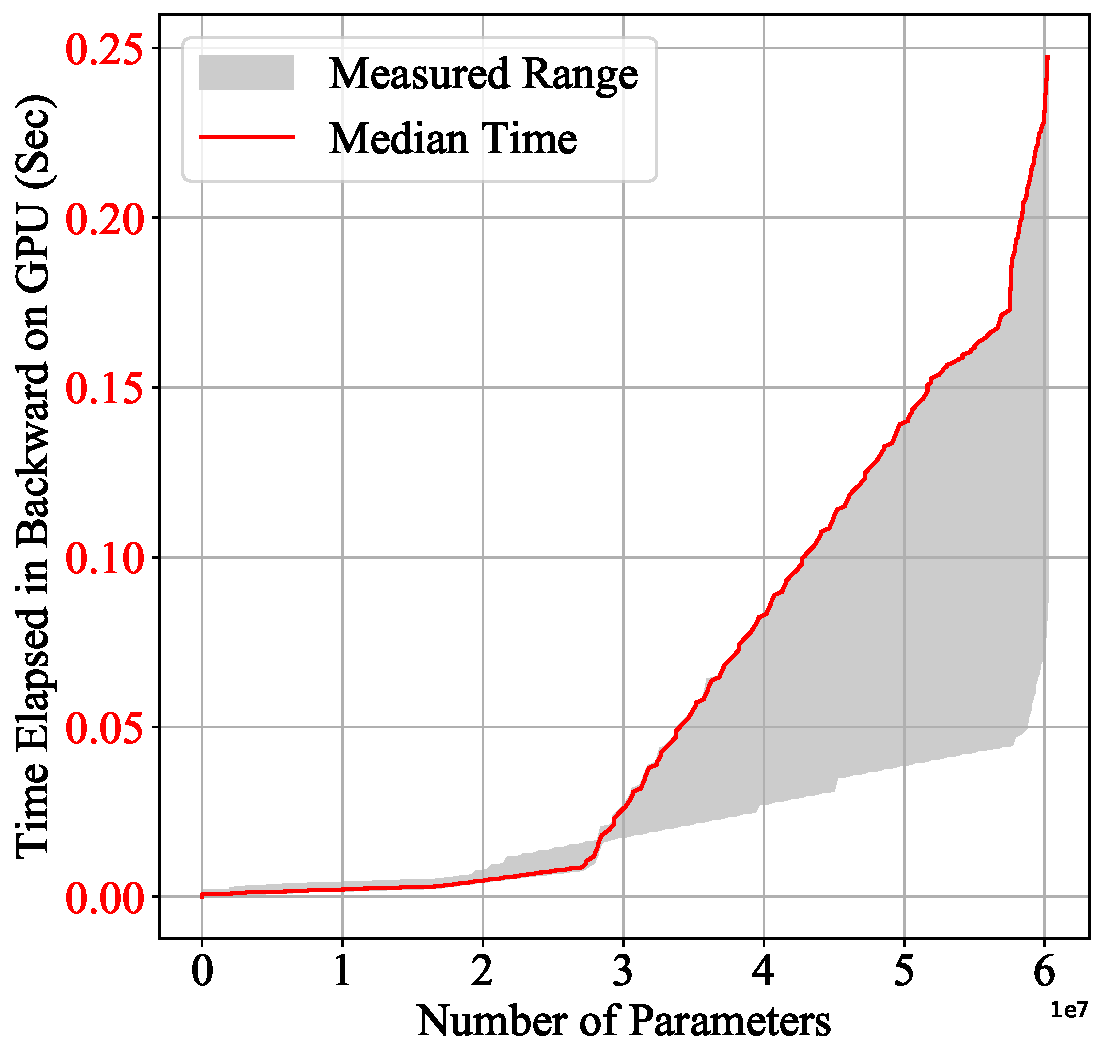
\includegraphics[width=\linewidth]{image/resnet152_gpu.pdf}
  (c) GPU
\end{minipage}
\begin{minipage}[r]{0.49\textwidth}
\flushright
\begin{minipage}[c]{0.96\textwidth}
  \centering
  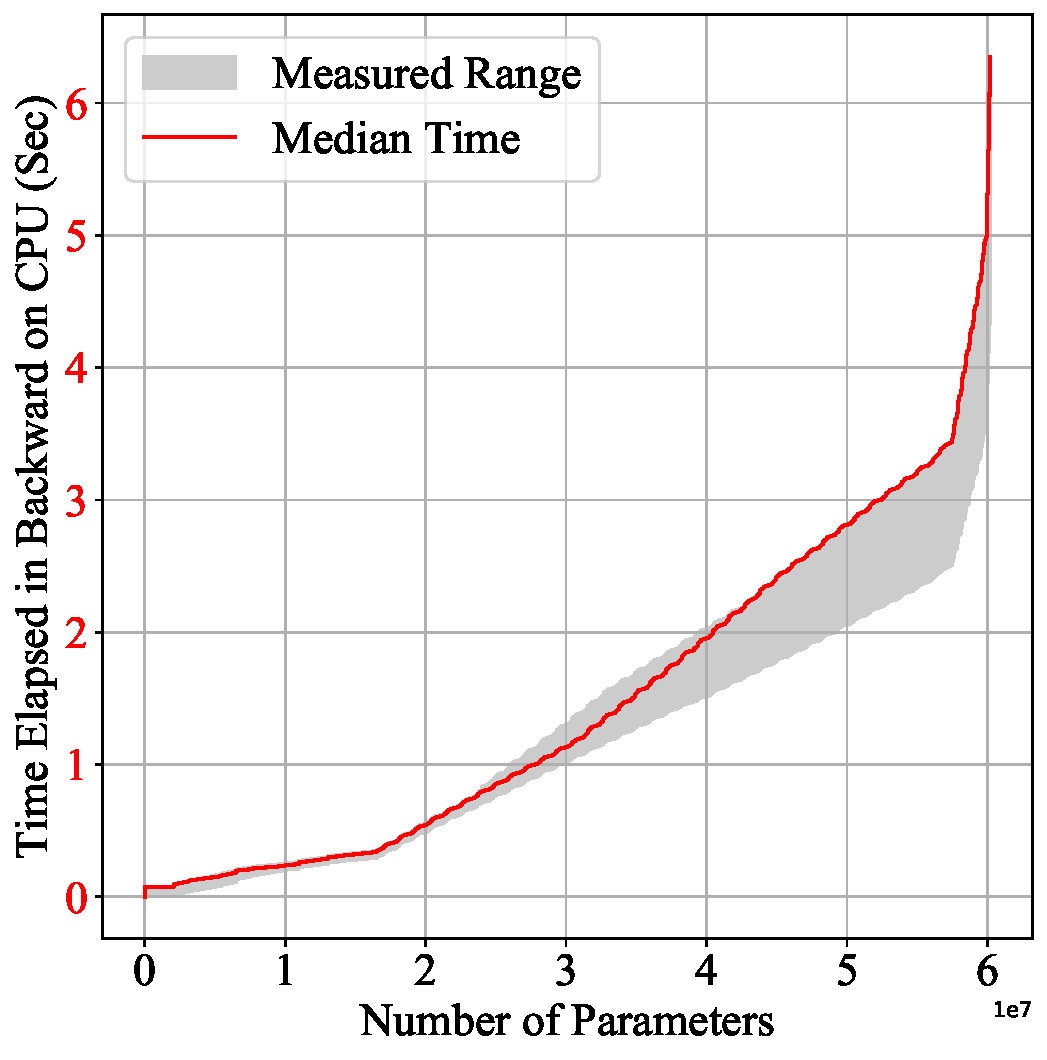
\includegraphics[width=\linewidth]{image/resnet152_cpu.pdf}
  (d) CPU
\end{minipage}
\end{minipage}
\end{minipage}
\vspace{-1em}
\caption{Communication vs Computation Delay}\label{fig:allreduce}
\vspace{-1em}
\end{figure}

\subsection{Gradient Reduction}\label{sec:reduction}



The gradient reduction algorithm in \code{DDP} has evolved over the past releases. To introduce the structure of the current implementation, let us start from a naive solution, gradually introduce more complexities, and land in the current version as of today in PyTorch v1.5.0. This will also explain how the same simple API described in Section~\ref{sec:api} allows us to install various performance optimization algorithms.



\subsubsection{A Naive Solution}

As mentioned in the beginning of Section~\ref{sec:design}, \code{DDP} guarantees correctness by letting all training processes (1) start from the same model state and (2) consume the same gradients in every iteration. The former can be achieved by broadcasting model states from one process to all others at the construction time of \code{DDP}. To implement the latter, a naive solution can insert a gradient synchronization phase after the local backward pass and before updating local parameters. However, the API shown in Section~\ref{sec:api} does not provide an explicit entry point for this phase as there is nothing between \code{backward()} and \code{step()}. Fortunately, the PyTorch autograd engine accepts custom backward hooks. \code{DDP} can register autograd hooks to trigger computation after every backward pass. When fired, each hook scans through all local model parameters, and retrieves the gradient tensor from each parameter. Then, it uses the \code{AllReduce} collective communication call to calculate the average gradients on each parameter across all processes, and writes the result back to the gradient tensor.

The naive solution is sufficient for our purposes, but there are two performance concerns. 
\vspace{-0.3em}
\begin{itemize}
    \item Collective communication performs poorly on small tensors, which will be especially prominent on large models with massive numbers of small parameters. 
    \vspace{-0.3em}
    \item Separating gradient computation and synchronization forfeits the opportunity to overlap computation with communication due to the hard boundary in between.
\end{itemize}
The following sections elucidates solutions to address the above two concerns.


\subsubsection{Gradient Bucketing}

The idea of gradient bucketing is motivated by the observation that collective communications are more efficient on large tensors. Fig.~\ref{fig:allreduce} (a) and (b) provide a quantitative view, which show the total execution time to \code{AllReduce} 60M \code{torch.float32} parameters with different numbers of parameters per \code{AllReduce}. To maximize the bandwidth utilization, \code{AllReduce} operations are launched asynchronously and block waiting on all of them together, mimicking \code{DDP}'s gradient reduction algorithm. The experiments are conducted on an NVLink~\cite{nvlink} enabled server with two NVIDIA Quadro GP100 GPUs. NCCL~\cite{nccl} \code{AllReduce} runs on CUDA input tensors directly, while Gloo~\cite{gloo} \code{AllReduce} runs on CPU input tensors to eliminate the overhead of copying between CUDA memory to CPU memory when using Gloo backend. The total communication time clearly decreases when using larger input tensors, for both NCCL and Gloo. Gloo reaches pinnacle speed at around 500K parameters per input tensor, while there is no clear saturation signal for NCCL on NVLink with even 20M-parameter GPU tensors. 

These experiments suggest that, instead of launching a dedicated \code{AllReduce} immediately when each gradient tensor becomes available, \code{DDP} can achieve higher throughput and lower latency if it waits for a short period of time and buckets multiple gradients into one \code{AllReduce} operation. This would be especially helpful for models with many small parameters. However, \code{DDP} should not communicate all gradients in one single \code{AllReduce}, otherwise, no communication can start before the computation is over. Fig.~\ref{fig:allreduce} (c) and (d) show the GPU and CPU backward computations time of a ResNet152~\cite{resnet} that contains roughly 60M parameters. The X axis is the number of ready gradients and the Y axis the time elapsed since the beginning of the backward pass. The backward on GPU takes about 250ms to complete, which is in the same order of magnitude as NCCL on NVLink. This conclusion also applies to Gloo and CPU backward. These measurements herald that, with relatively small bucket sizes, \code{DDP} can launch \code{AllReduce} operations concurrently with the backward pass to overlap communication with computation, which would make a difference in per iteration latency. 

\subsubsection{Overlap Computation with Communication}\label{sec:overlap}

The \code{AllReduce} operation on gradients can start before the local backward pass finishes. With bucketing, \code{DDP} only needs to wait for all contents in the same bucket before launching communications. Under such settings, triggering \code{AllReduce} at the end of the backward pass is no longer sufficient. It needs to react to more frequent signals and launches \code{AllReduce} more promptly. Therefore, \code{DDP} registers one autograd hook for each gradient accumulator. The hook fires after its corresponding accumulator updating the gradients, and will inspect the bucket it pertains. If hooks of all gradients in the same buckets have fired, the last hook will trigger an asynchronous \code{AllReduce} on that bucket. 

\begin{figure}
\centering
  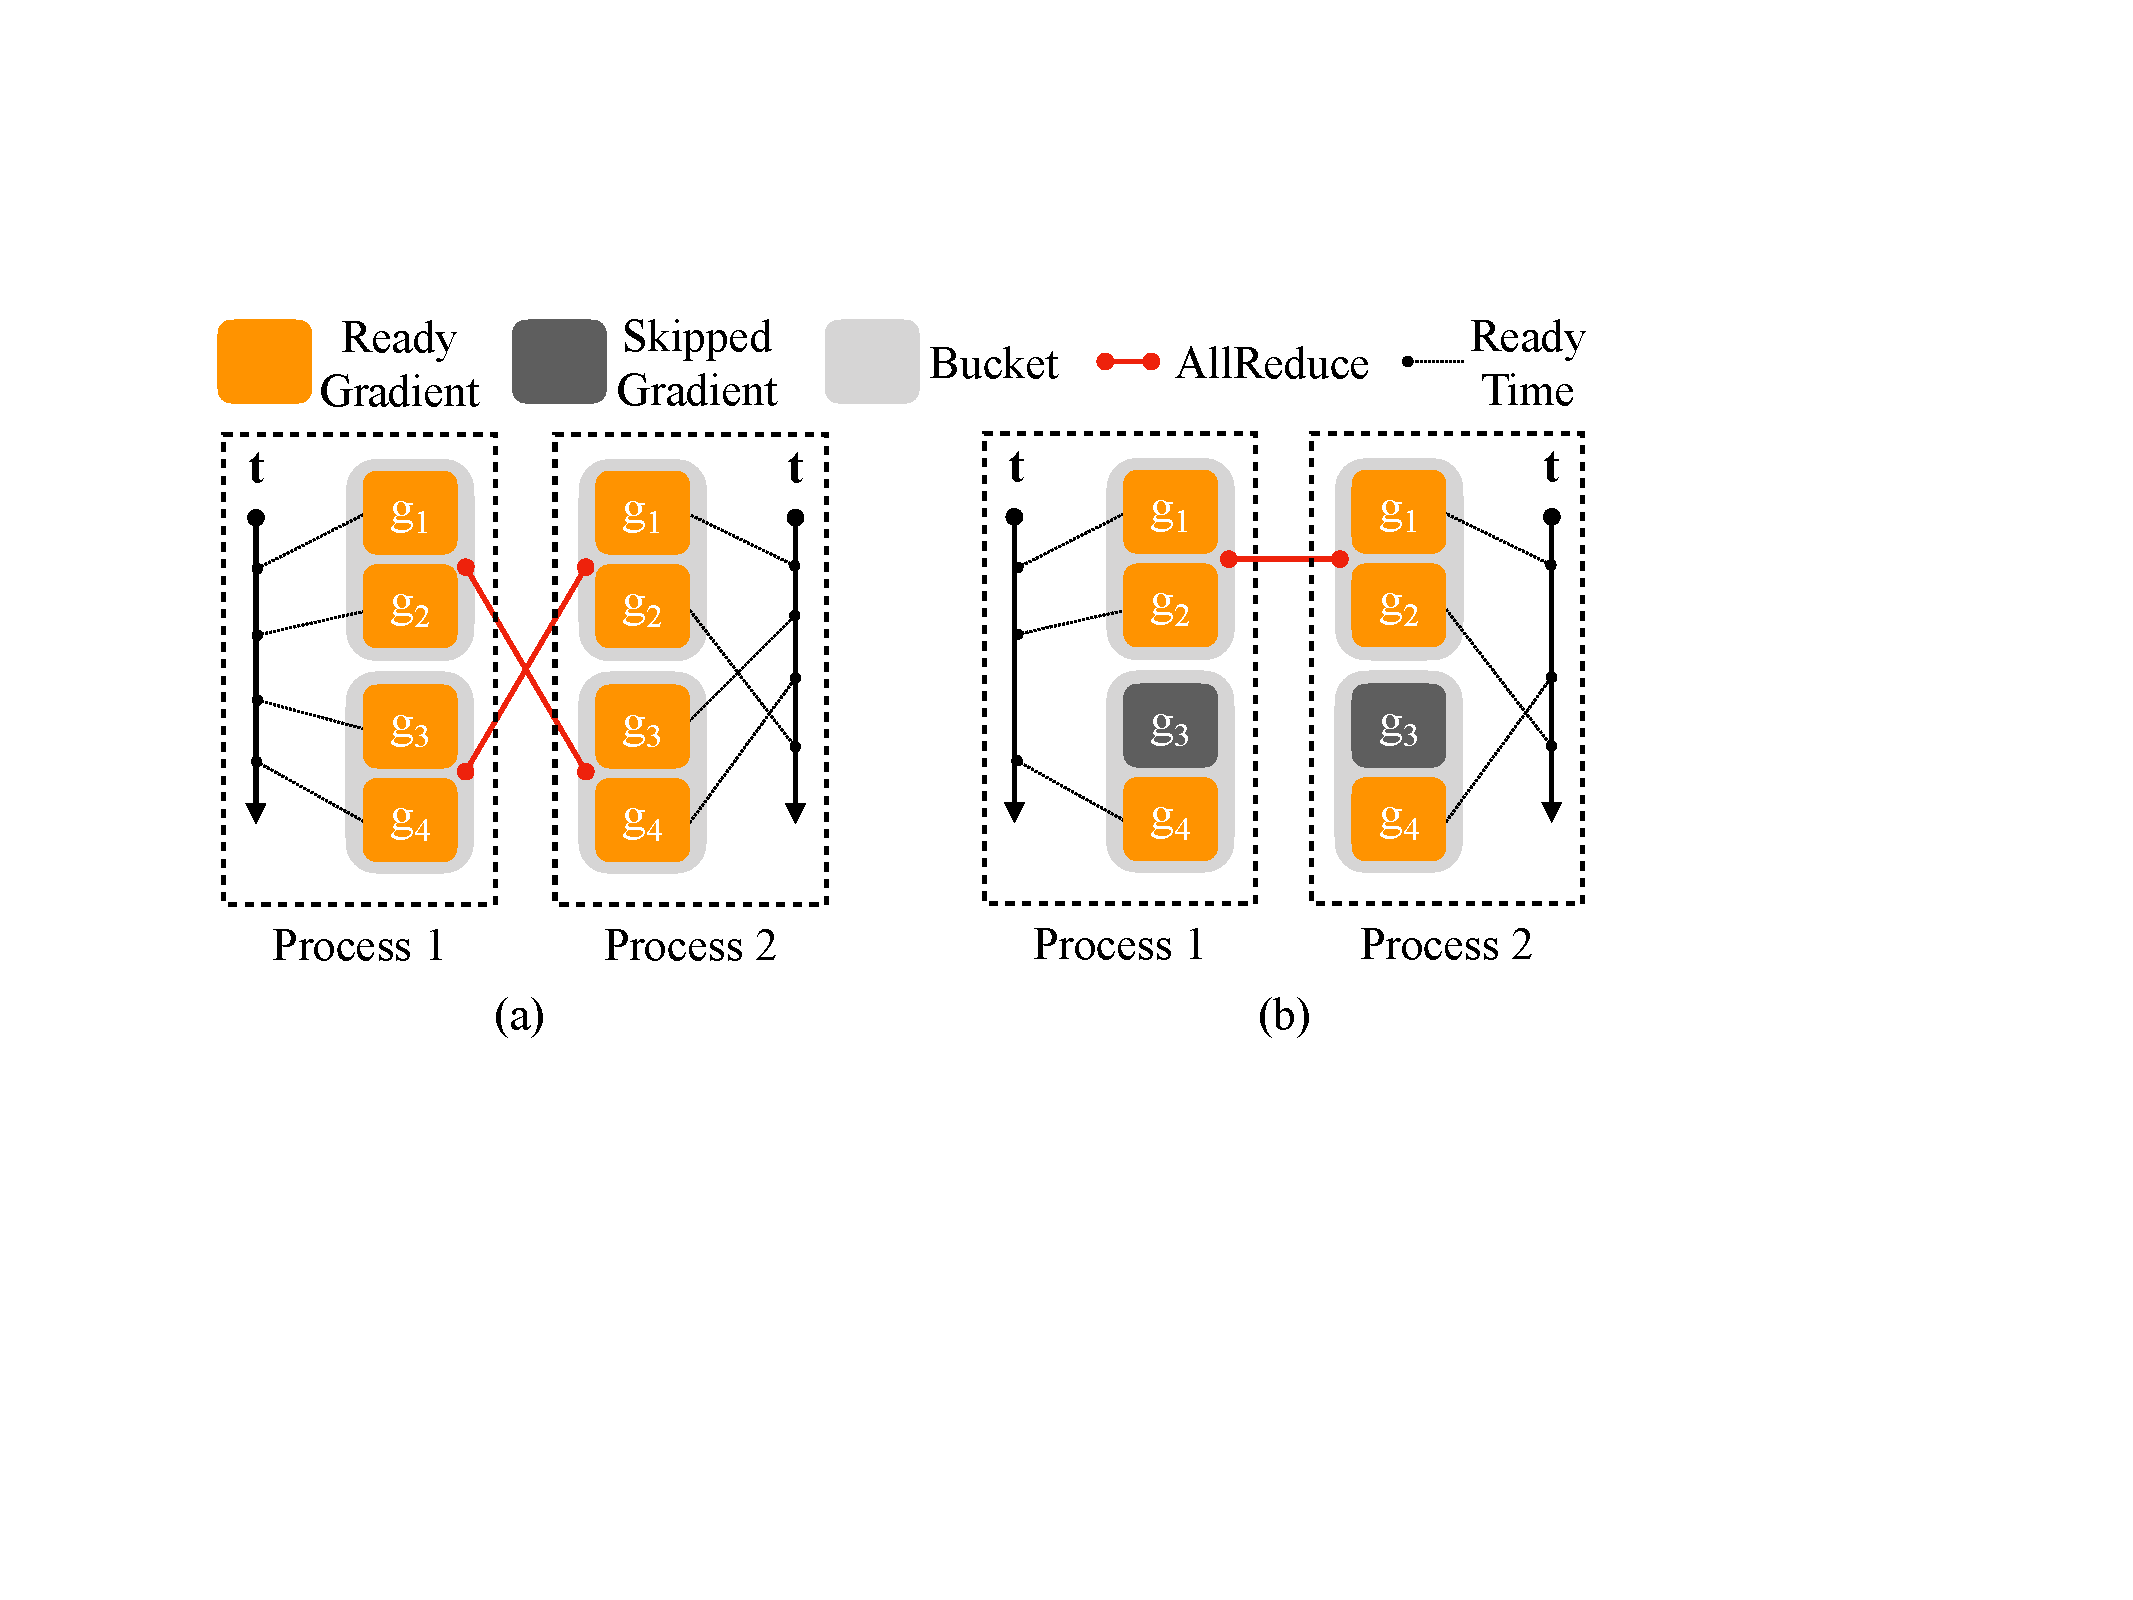
\includegraphics[width=0.9\linewidth]{image/caveats.pdf}
  \vspace{-1em}
  \caption{Gradient Synchronization Failures}\label{fig:caveats}
  \vspace{-1.5em}
\end{figure}

% New
Two caveats require caution. First, the reducing order must be the same across all processes, otherwise, \code{AllReduce} contents might mismatch, resulting in incorrect reduction result or program crash. However, PyTorch dynamically builds the autograd graph in every forward pass, and different processes might not agree on the gradient ready order. Fig.~\ref{fig:caveats}~(a) shows one example, where the two vertical axes represent time and dotted lines indicate when a gradient is ready. In process 1, the four gradients are computed in order, but the gradient $g_2$ are computed after $g_3$ and $g_4$ on process 2. In this case, if all processes \code{AllReduce} buckets as soon as they become ready, the \code{AllReduce} content would mismatch. Therefore,
%
all processes must use the same bucketing order, and no process can launch \code{AllReduce} on bucket \code{i+1} before embarking bucket \code{i}. If bucket \code{0} is the last one that becomes ready, there is no way that communication can overlap with computation. PyTorch v1.5.0 addresses this problem by using the reverse order of \code{model.parameters()} as the bucketing order, assuming that, layers are likely registered according to the same order as they are invoked in the forward pass. Hence, the reverse order should approximately represent the gradient computation order in the backward pass. Admittedly, this is not a perfect solution, but is an approximation that we can rely on with minimum engineering overhead.

Second, it is possible that one training iteration only involves a sub-graph in the model and the sub-graph can be different from iteration to iteration, meaning that some gradients might be skipped in some iterations. However, as gradient-to-bucket mapping is determined at the construction time, those absent gradients would leave some buckets never seeing the final autograd hook and failing to mark the bucket as ready. As a result, the backward pass could hang. 
% New
Fig.~\ref{fig:caveats}~(b) shows an example, where the parameter corresponding to gradient $g_3$ is skipped in one iteration, leading to the absent of the ready signal for $g_3$.
%
To address this problem, \code{DDP} traverses the autograd graph from the output tensors of the forward pass to find all participating parameters. The readiness of those participating tensors is a sufficient signal to conclude the completion of the backward pass. Therefore, \code{DDP} can avoid waiting for the rest of the parameter gradients by proactively marking them ready at the end of the forward pass. Note that, this change does not prevent us from developing non-intrusive APIs, because application directly invokes the \code{forward} function on \code{DDP} and hence \code{DDP} can easily insert this step in its member function. 

\vspace{-0.8em}

\begin{algorithm}
\footnotesize
\caption{DistributedDataParallel}\label{algo:reduction}
\KwIn{Process rank $r$, bucket size cap $c$, local model $net$}
\SetKwFunction{constructor}{constructor}
\SetKwFunction{forward}{forward}
\SetKwFunction{hook}{autograd\_hook}
\SetKwProg{Fn}{Function}{:}{}
\Fn{\constructor{net}}{
\If{r=0}{
broadcast $net$ states to other processes\\
}
init buckets, allocate parameters to buckets in the reverse order of net.\text{parameters()}\\
\For{p \textbf{in} net.parameters()}{
    acc $\leftarrow p.\text{grad\_accumulator}$\\
    acc $\rightarrow \text{add\_post\_hook}(\text{autograd\_hook})$\\
}
}
\Fn{\forward{inp}}{
    out = $net$(inp)\\
    traverse autograd graph from out and mark unused parameters as ready\\
    \text{\textbf{return}} out
}
\Fn{\hook{param\_index}}{
get bucket $b_i$ and bucket \emph{offset} using param\_index\\
get parameter $var$ using \emph{param\_index}\\
view $\leftarrow b_i.narrow($\emph{offset}, $var.size())$\\
view.copy\_(var.grad)\\
\If{all grads in $b_i$ are ready}{
    mark $b_i$ as ready\\
}
launch AllReduce on ready buckets in order\\
\If{all buckets are ready}{
    block waiting for all AllReduce ops\\
}
}
\end{algorithm}

\vspace{-0.8em}


Algorithm~\ref{algo:reduction} presents the pseudo-code of \code{DDP}. The constructor contains two major steps, broadcasting model states and installing autograd hooks. \code{DDP}'s \code{forward} function is a simple wrapper of the local model's \code{forward}, and traverses the autograd graph to mark unused parameters at the end. The \code{autograd\_hook} takes the internal parameter index as input, which helps to find the parameter tensor and its belonging bucket. It writes the local gradient to the correct offset in the bucket and then launches the asynchronous \code{AllReduce} operation. There is an additional finalizing step omitted in the pseudo-code that waits for \code{AllReduce} operations and writes the value back to gradients at the end of the backward pass.  Fig.~\ref{fig:ddp} elucidates how \code{DDP} interacts with the local model during the forward and backward passes.

\begin{figure}
\centering
  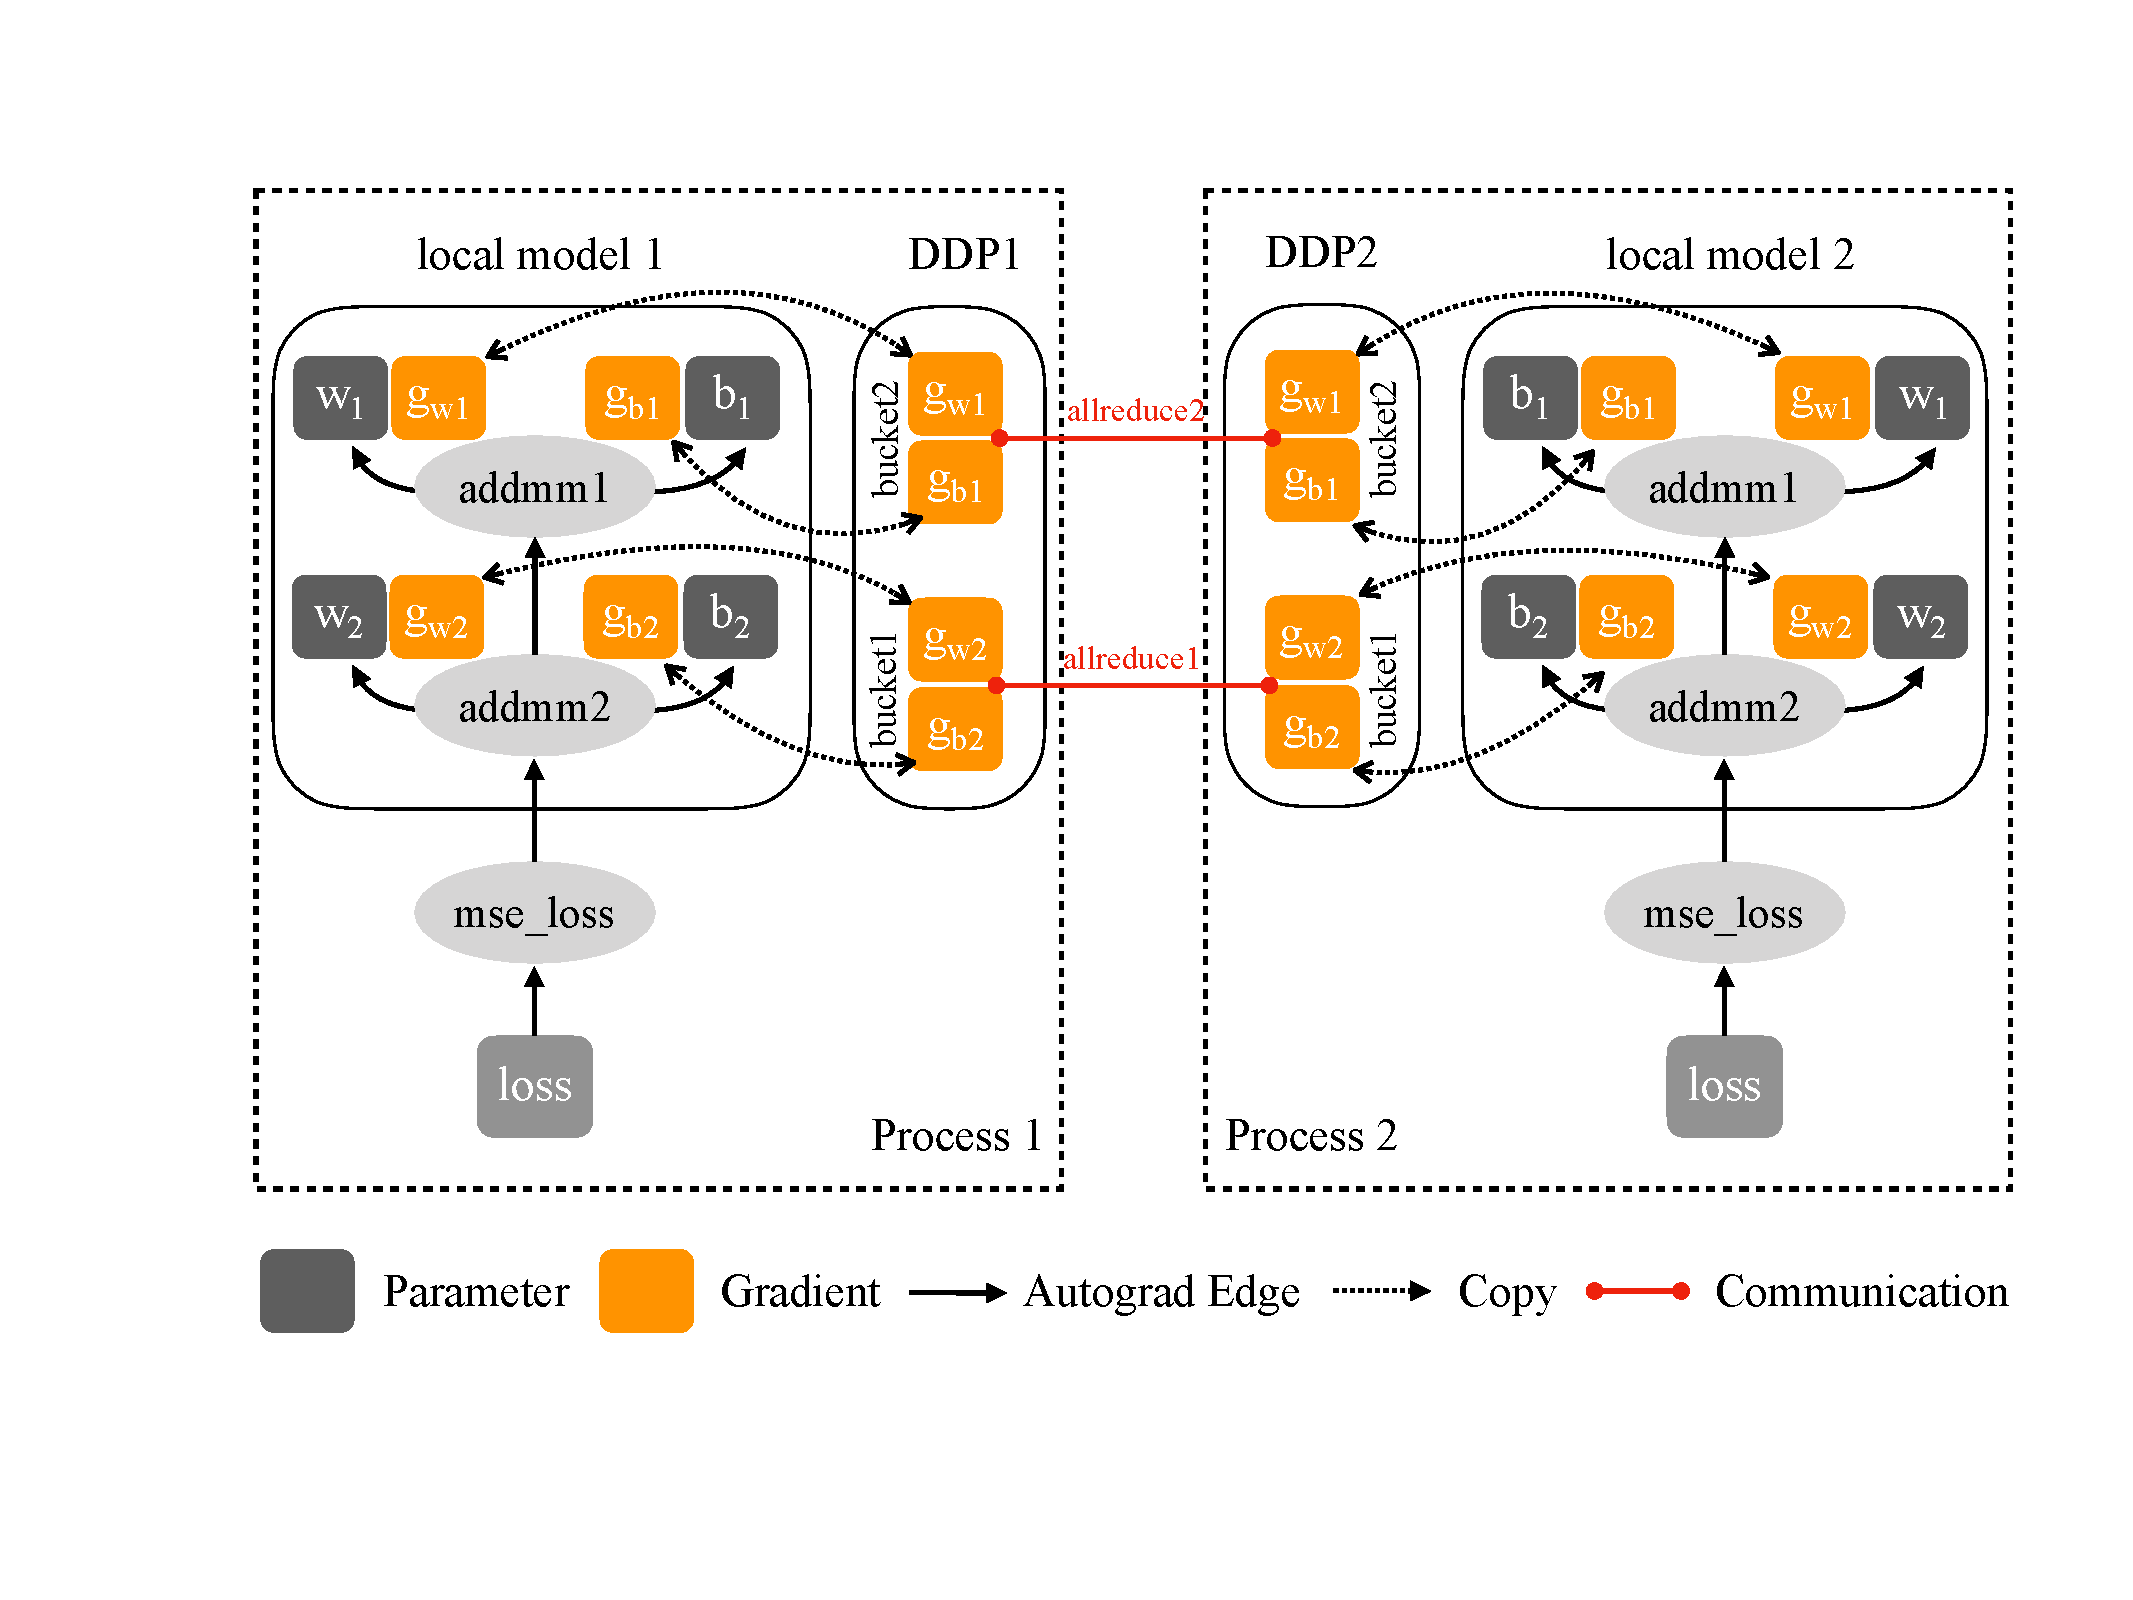
\includegraphics[width=0.9\linewidth]{image/ddp.pdf}
  \vspace{-1em}
  \caption{Distributed Gradient Reduction}\label{fig:ddp}
  \vspace{-1.5em}
\end{figure}




The above solution works for most use cases. However, as \code{DDP} always computes the average of all gradients and writes them back to parameter \code{.grad} field, an optimizer cannot distinguish whether a gradient has participated in the last backward pass or not. Due to the decoupled design of \code{DDP} and the optimizer, there is no side channel for \code{DDP} to allude that information to the optimizer. Without this information, the training process could suffer from regressions on model accuracy, \emph{e.g.}, when the optimizer uses gradient absence information to skip updating momentum values. To tackle this problem, \code{DDP} should only touch gradients that are indeed involved in the backward pass. Nevertheless, this information cannot be extracted from the local autograd graph alone, because locally absent gradients might still be involved in the forward/backward pass in a peer \code{DDP} process. Therefore, \code{DDP} uses a bitmap to keep track of local parameter participants and launches one additional \code{AllReduce} to collect globally unused parameters. Unfortunately, \code{DDP} cannot coalesce this bitmap into other gradient \code{AllReduce} operations due to the potential mismatch in element types. Such additional overhead only materializes when the application explicitly tells \code{DDP} to look for unused parameters, and hence the price is only paid when necessary. 


\subsubsection{Gradient Accumulation}\label{sec:accumulation}

One common technique to speed up distributed data parallel training is to reduce gradient synchronization frequencies. Instead of launching \code{AllReduce} in every iteration, the application can conduct $n$ local training iterations before synchronizing gradients globally. This is also helpful if the input batch is too large to fit into a device, where the application could split one input batch into multiple micro-batches, run local forward and backward passes on every micro-batch, and only launch gradient synchronization at the boundaries of large batches. Theoretically, this should produce the same results as if all data in the large batch is processed in one shot, as gradients will simply be accumulated to the same tensor. However, this conflicts with the gradient reduction algorithm discussed in Section~\ref{sec:overlap} to some degree. That algorithm would mark unused parameters as ready at the end of every forward pass, while those unused parameters in one iteration still could participate in subsequent iterations. Moreover, \code{DDP} cannot distinguish whether the application plans to immediately invoke \code{optimizer.step()} after backward or accumulate gradients through multiple iterations. Therefore, we need to introduce one additional interface (\emph{i.e.}, \code{no\_sync}) for this use case. Below is an example code snippet.
\begin{lstlisting}[language=Python]
ddp = DistributedDataParallel(net)
with ddp.no_sync():
  for inp, exp in zip(inputs, expected_outputs):
    # no synchronization, accumulate grads
    loss_fn(ddp(inp), exp).backward()  
# synchronize grads
loss_fn(ddp(another_inp), another_exp).backward()  
opt.step()
\end{lstlisting}
Under the hood, the implementation for \code{no\_sync} is very simple. The context manager just toggles a flag on entering and exiting the context, and the flag is consumed in the \code{forward} function of \code{DDP}. In \code{no\_sync} mode, all \code{DDP} hooks are disabled, and the first backward pass out of the context will synchronize the accumulated gradients altogether. The information of globally unused parameters also accumulates in the bitmap, and serves when the next communication takes place.